\documentclass[pdftex,bibtotocnumbered,idxtotoc,11pt]{scrartcl}
%\documentclass[a4paper]{article}
\usepackage{amsmath,amsfonts}
\usepackage{times,latexsym}
\usepackage{xcolor,graphicx,fancybox,wrapfig}
\usepackage{url,acronyms,myref,locutor}
\usepackage{wasysym}
\usepackage{listings}
\usepackage{lstomdoc}
\usepackage{xmlindex}
\usepackage[hide]{ed}
\usepackage[margin={2.5cm,2.5cm,1.5cm,1.5cm}]{geometry}


% Load this last!
\usepackage{hyperref}
%%

\lstset{float=htb,columns=flexible,frame=lines,language=[omdoc]XML,basicstyle=\scriptsize,
        indexstyle=\indextt,indexstyle=[1]\indexelement,indexstyle=[2]\indexattribute,
        numbers=left,stepnumber=5,numberstyle=\tiny,showstringspaces=false}

\newcommand{\PC}{\mathcal{PC}}
\renewcommand{\mod}{\operatorname{mod}}

\def\name#1{{{\small{\sc{#1}}}}}

\makeatletter
\renewcommand\paragraph{\@startsection{paragraph}{4}{\z@}%
{1.25ex \@plus1ex \@minus.2ex}%
{-1em}%
{\setlength{\parfillskip}{\z@ \@plus 1fil}%
\raggedsection\normalfont\sectfont\nobreak
\size@paragraph\nobreak}}
\makeatother

\title{Documents with flexible Notation Contexts as Interfaces to Mathematical Knowledge}
\author{Michael Kohlhase, Christine M{\"u}ller, Normen M{\"u}ller\\ 
  Computer Science, Jacobs University Bremen, Germany\\
  {\small\url{m.kohlhase/c.mueller/n.mueller@jacobs-university.de}}}
\date{}

\begin{document}
\maketitle

\begin{abstract}\vspace*{-.7cm}
  In this paper we explore the use of documents as interfaces to mathematical
  knowledge. We propose an augmented document model that facilitates the explication of a
  document's notation context, i.e.\ the selection of appropriate presentations for all
  symbols in the document. By separating the notation context from the structure and
  content of a document, we aim at identifying the author's selection of notation, i.e.\
  his notation practices. This facilitates both, the identification of communities of
  practice ({\cop}) that share specific notation preferences and, conversely, the
  adaptation of documents to the notation preferences of identified {\cop}s, e.g.\ groups
  of readers and co-authors. Furthermore, explicating a document's notation context allows
  for referencing and, particularly, reusing contexts, which reduces the author's workload
  during the authoring process.
\end{abstract}

\section{Introduction}\label{sec:intro} 

In this paper we will re-evaluate the concept of a document in the age of digital
media. Since the development of writing, documents have become one of the primary means of
passing on knowledge. If we take the view that knowledge is a state of the (human) mind
where concepts and experiences are highly interlinked, and interpret ``documents'' broadly
to include spoken language or action sequences played out\footnote{After all, these can be
  captured by the digital media.}, then we can see that documents are almost the only
means to communicate knowledge: quite literally, {\emph{documents are interfaces to
    knowledge}}. Here, we will look at {\emph{mathematical documents}} as interfaces to
{\emph{mathematical knowledge}}, since they have special complexities that reveal the
underlying nature of documents and knowledge.

Before Gutenberg, the notion of a document was relatively clear: a document is a physical
object created by applying ink to paper or parchment for the purposes of transporting
information in the form of images or written language. With the invention of letterpress
printing, the production of verbatim copies became so simple, that we have to distinguish
two aspects of documents: the {\emph{information object}} (IO, i.e.\ the common
information conveyed by all copies), and the {\emph{physical object}} (PO, e.g.\ the
book), which are distinct: for instance, if you destroy one of the physical books (e.g.\
by burning it), then you do not necessarily destroy the information object which can live
on in other copies. In the age of electronic typesetting, the picture becomes more complex
still, since the {\emph{digital representation}} (DR) of a document appears; it is
situated somewhere between the IO and the PO, and is distinct from both. Moreover, the
perceived one-to-one correspondence between the IO and the PO becomes tenuous, since the
DR is structurally different from the PO (e.g.\ the screen presentation for printout).
Consider for instance document parts like the table of contents or index in {\LaTeX},
which are spread over the DR and are assembled during the formatting process that creates
the PO. We will neglect the difference between the DVI file and the printout for the sake
of this argument, but make use of the fact that we can also use the term PO for
``{\emph{presentation object}}'' which includes the former without excluding the
latter. Generalizing the IO-PO correspondence also allows to re-interpret the IO as the
knowledge conveyed by the document and try to approximate it with a {\emph{content
    representation}} (CR), that tries to capture the structure of the knowledge rather
than the structure of the PO. We see first steps in this direction already in {\LaTeX} and
{\sc{sgml}}, which strive to separate {\emph{function}} from {\emph{form}} in documents
and employ styling mechanisms to compute the document form (i.e.\ the PO) from the
CR. This trend finds its (current) conclusion in markup languages like
{\openmath}~\cite{BusCapCar:2oms04} and {\mathml}~\cite{CarIon:MathML03} for mathematical
formulae and {\omdoc}~\cite{Kohlhase:omdoc1.2} for mathematical documents which offer
means to ``identify the structure, the meaning of text fragments, and their relations to
other knowledge''~\cite{Kohlhase:omdoc1.2}.

In the context of such languages and dynamic presentation media (e.g.\ on the screen), we
can now dream about ``{\emph{active documents}}'', where we can interact with a document
directly, e.g.\ instantiating a formula with concrete values or graphing a function to
explore it or ``{\emph{living/evolving documents}}'' which monitor the change of knowledge
about a topic. All of these developments can strengthen the role of documents as
interfaces to mathematical knowledge by empowering the reader in her interaction with the
content, but considerably weaken our understanding of what a ``document'' might be.

In this paper, we will drill in on the intuition that a ``document'' should be an object,
whose extent and context are fixed by a ``publication'' process, and which contains enough
information that a PO can be generated for it (e.g.\ for printing into a ``pre-Gutenberg''
document). We will use the process of presenting mathematical formulae as a razor to
distinguish conceptual aspects documents and propose a novel document architecture, which
we will develop concretely in the context of our {\omdoc} format.

% The markup of structure and content of documents in a form that can be understood,
% interpreted, and used by machines has facilitated the development of various
% mathematical applications. 
% For example, the following systems facilitate the maintenance, sharing, creation, and
% search of information by document markup based on {\omdoc}: The \textit{change
% management service {\locutor}}~\cite{locutor:web} uses the explicit markup of
% structure and content to ensure the consistent reuse, modification and creation of
% content for arbitrary structured documents. The \textit{eLearning environment
% {\activemath}}~\cite{MAF+01} generates user-centered educational courses from an
% {\omdoc} repository and a respective didactic structure.  The \textit{semantic wiki
% {\swim}}~\cite{Lange:swmkm-tr07} supports the collaborative creation and browsing of
% mathematical content. In addition, the \textit{search engine
% {\emph{MathWebSearch}}}~\cite{KohSuc:mwssse07} crawls various repositories of Content
% {\mathml} and {\openmath} formulae to retrieve specific mathematical knowledge, i.\,e.\
% formulae.

\paragraph{Presenting Mathematical Formulae} In~\cite{Naylor:conversion} Naylor and Watt
present an approach based on meta style sheets that was deployed in the \emph{Notation
  Selection Tool}~\cite{NotSelectTool:web}: The approach utilizes a {\mathml}-based markup
of arbitrary notations in terms of their content and presentation and, based on the manual
selection of users, generates user-specific {\xslt} style sheets~\cite{W3C:xslt2} for the
adaptation of documents. In~\cite{ManLib:apo05} Manzoor et al.\ emphasize the need for
maintaining uniform and appropriate notations in collaborative environments, in which
various authors contribute mathematical material. They address the problem by providing
authors with respective tools for editing notations as well as by developing a framework
for a consistent presentation of symbols.

In this paper we propose the markup of the {\emph{notation context}} of a document, i.e.\
the explication of the selected presentation for symbols by the author. By separating the
notation context from the content and structure of the document, we present an alternative
approach that reduces the workload of authors and supports the comprehensibility of
documents by readers: For example, one could imagine that documents could be easily
switched to the notation context preferred by a community of practice
({\cop})~\cite{Wen05}, e.g.\ groups of readers and co-authors. Alternatively, authors
could be enabled to reuse the notation contexts of other documents or the notation
preference of a specific user or
{\cop}.%, which would reduce the workload during the authoring process.

\paragraph{The Document/ Knowledge Model in {\omdoc}:}
The semantic markup language {\omdoc}1.2. contains two {\omdoc} types\footnote{The
  {\omdoc} group does do not claim to have invented this concept, it is part of the {\xml}
  folklore and can already be found e.g.\ in~\cite{vd04:nc}. But the {\omdoc} format
  probably implements this idea in the cleanest way.} in order to mark up the knowledge
contained in a mathematical document and its structure: Content {\omdoc}s are
``knowledge-centered documents that contain the knowledge conveyed in a
document''~\cite{Kohlhase:omdoc1.2}. In contrast, narrative {\omdoc}s are used to
``reference the knowledge[-centered documents] and add the theoretical and didactic
structure of a document''~\cite{Kohlhase:omdoc1.2}. The combination of the narrative
structure and the (mathematical) content of a document as the formal representation of a
document model, has been defined by Normen M\"uller as {\narcon}s, i.e.\ two-dimensional
graphs consisting of a \textbf{nar}rative layer and a \textbf{con}tent
layer~\cite{NRM:lwa06}. Several terms have been created to denote knowledge in the content
layer of a {\narcon}: Michael Kohlhase~\cite{Kohlhase:omdoc1.2} uses the term
\textit{knowledge item}, while Normen M\"uller proposes the term {\emph{information
    units}} or {\infom}s, i.\,e.\ ``tangible/visual text fragments potentially adequate
for reuse, constituting the content of documents''~\cite{NRM:lwa06}. We use the term
{\infom} to refer to {\emph{fragments of content}} that are represented in
{\emph{Content}} {\omdoc}.  {\infom}s are stored in an {\omdoc} repository, which we call
{\emph{content commons}} according to the terminology of the educational knowledge
repository {\connexions}~\cite{cnxweb}. In this paper we revise our previous definition of
documents and present an augmentation of {\narcon}s (cf.~section~\ref{sec:docmodel}).
%, which created this term to denote a common collection of mathematical content.

%-----------------------------------------------------------------------------------------
\paragraph{Notation Context and Notation Practice:}
The {\emph{notation context}} of a document shall be defined as a mapping of symbols to
presentations. The selection of respective presentation for symbols highly depends on the
author's {\emph{notation practice}}, i.e.\ his individual way of selecting notations,
which he acquires throughout his life and which is influenced by a number of factors.

Various researchers have addressed the challenge of identifying and describing
mathematical practice. In~\cite{ESmStW:Notation} Watt and Smirnova introduce possible
{\emph{reasons}} for multiple notations of the same mathematical concept, namely
{\emph{area of application}}, {\emph{national conventions}}, {\emph{level of
    sophistication}}, the \textit{mathematical context}, and the {\emph{historical
    period}}: For example, to introduce an imaginary unit, a mathematician uses the symbol
$i$. In contrast, an electrical engineer uses $j$ to avoid confusion with the symbol $I$
for electric current. $i$ and $j$ are two alternative presentation for the symbol
``imaginary unit''. Hence, the {\emph{notation context}} of a mathematical document will
most likely refer to the notation $i$, while the notation selected for a document by an
electrical engineer refers to $j$. Based on the {\emph{national convention}} we
distinguish notations that are commonly used in different language. For example, a German
researcher presents the symbol ``binomial coefficient'' with the notation ${n \choose
  k}$. In contrast, a Russian researcher uses the alternative presentation $C_{k}^n$,
while a French researcher will most likely use $C_{n}^k$.

In contrast to the five {\emph{``reasons''}} in~\cite{ESmStW:Notation}, the {\omdoc}-based
eLearning environment {\activemath}~\cite{ManLib:apo05} distinguishes four
{\emph{``contexts'' categories}} that influence the adaptation of notations, namely
{\emph{language}}, {\emph{different patterns of the argument}}, the {\emph{author's
    style}}, and {\emph{notations of the same collection}}. For example, depending on his
individudal style, an author will use $a/b$ or $a:b$ (cf.~\cite{ManLib:apo05}). In
addition, the {\activemath} group specified a prioritization of notation collections,
which we referred to as {\emph{notation contexts}}: {\emph{system defaults}},
{\emph{author}}, {\emph{book}}, {\emph{group}}, and {\emph{individual}} style (highest
priority). Furthermore, in {\activemath} authors can annotate different layout preferences
for notations, such as {\emph{color}}, {\emph{font}}, or {\emph{border}}, which shall also
be considered parts of the notation practice.

%-----------------------------------------------------------------------------------------
\paragraph{Communities of Practice:}
In~\cite{KohKoh:copmem06} Andrea Kohlhase and Michael Kohlhase propose the application of
the economic theory of {\emph{communities of practice ({\cop})}}~\cite{Wen05} to the area
of mathematics. According to their discussions, {\emph{mathematical practice}} is
{\emph{inscribed}} into documents, e.\,g.\ by selecting specific notations or referencing
other mathematical publications. Analyzing a {\emph{collection of documents}} will
potentially lead to {\emph{clusters of shared practices}}, i.e. {\emph{communities of
    practice}}, that define the mathematical practice of researchers. For example, the
participants of the MathUI Workshop establish a community of notation practice by adapting
to the notation of fellow researchers and, vice versa, by influencing the community with
their individual habits. The longer a researcher takes part in the annual MathUI Workshop,
the more likely he will adapt to this set of shared notations, hence moving from the outer
border of the MathUI {\cop} to the inner parts. However, \cite{KohKoh:copmem06} further
emphasize the problem of {\emph{inscribing practices}}, e.\,g.\ by {\emph{enforcing}} the
use of specific notations in an editor, and call for the implementation of workflows that
preserve the {\emph{fluid movement}} in and between {\cop}s.

This paper aims at resuming the discussion on mathematical {\cop}s and takes one step
towards a {\emph{{\cop} model}} that preserves the {\emph{dynamics}} and
{\emph{flexibility}} of {\emph{mathematical communities}} in terms of their
{\emph{notation practice}} (cf.\ section~\ref{sec:docmodel}).


%%%%%%%%%%%%%%%%%%%%%%%%%%%%%%%%%%%%%%%%%%%%%%%%%%%%%%%%%%%%%%%%%%%%%%%%%%%%%%%%%%%%%%%%%%
\section{Modeling the Notation Context in OMDoc}\label{sec:docmodel}

We have extended our {\narcon} model by a third dimension --- the presentation layer and
developed a concrete syntax for inclusion in {\omdoc}2.0: In {\omdoc}1.2, the root element
{\element{omdoc}} does double duty: encapsulating content- and narrative- and mixed
documents without an elaborated mechanism that allows to distinguish between the
cases. Moreover, the document structure is marked up by the {\element{omgroup}} element
that has the same content model as the {\element{omdoc}} element. In the proposed document
representation, we bid farewell to the illusion that we can represent narrative and
content structure in one document, and make the three dimensions of a document explicit.
Documents will be structured by {\element{omdoc}} elements which have three optional
children: a {\element{narrative}} element specifying the narrative structure of the
document, a {\element{content}} caching its {\infom}s, and a
{\element{pcontext}}\footnote{The element is named \underline{p}resentation
  \underline{context} since it will also be used to specify further presentation-specific
  contexts besides the notation contexts, e.\,g.\ layout preferences such as color or
  fonts. For the further course of the paper, both terms, notation and presentation
  contexts, are used synonymously.} for explicating the notation context of the
document. We propose that the {\attribute{type}{omdoc}} attribute on the {\element{omdoc}}
element be generated from the {\emph{document ontology}}~\cite{NRM:wp1:07} of {\omdoc}.

The following RelaxNG~\cite{Vlist:Relaxng} grammar summarizes the proposed document
structure.

\begin{lstlisting}[mathescape,numbers=none]
id.att          = attribute xml:id {xsd:ID}
omdoc           = element omdoc {id.att?,attribute type{xsd:NCName}, pcontext?, narrative?, content?}
pcontext        = element pcontext {id.att?,attribute base list {xsd:anyURI*},ref*}
narrative       = element narrative {id.att?,narrative.class*}
content         = element content {content.class*}
narrative.class = metadata|omdoc|ref|tableofcontents|authorindex|$\ldots$
content.class   = omtext|definition|theory|$\ldots$
\end{lstlisting}

The {\element{narrative}} element specifies the structure of a document via
{\element{omdoc}} elements (e.\,g.\ for chapters or sections) and via {\element{ref}}
elements that reference (i.e.\ include) document fragments from the {\emph{document
    commons}}\footnote{A {\emph{document commons}} is a repository of documents, e.\,g.\
  in {\omdoc} format.} or {\infom}s from the sibling {\element{content}} element. These
can be freely inter mixed with special narrative elements for tables of content, indices,
etc.

The {\element{content}} element is used to {\emph{cache}} content of the document that is
referenced in the {\element{narrative}} elements of the document. For example, an
{\element{omtext}} element that already exists in the {\emph{content commons}}, can be
referenced in the {\element{narrative}} element and may optionally be copied to the
{\element{content}} element. Alternatively, the author can write a new {\element{omtext}}
element himself, which is then added to the {\element{content}} element and eventually
added to the {\emph{content commons}}\footnote{For now we assume that the author manually
  references the existing elements from the \textit{content commons}, i.e.\ by indicating
  the respective URI. Also, when adding new elements to the content commons (that
  potentially already exist in the repository), these are currently not matched with the
  exiting ones but simply stored as new entries. In the near future, the consistent
  referencing of existing elements as well as the alignment of new/ modified elements
  among existing ones will be managed automatically.}.

The {\element{pcontext}} element is a collection of one or more references to
{\element{presentation}} elements in the sibling {\element{content}} element or
{\emph{content commons}}. The optional {\attribute{base}{pcontext}} attribute contains a
whitespace-separated list of URIs pointing to {\element{pcontext}} of other {\narcon}s,
hence it can be used to inherit presentation contexts. The effective presentation context
is computed by cascading (left-to-right) the effective presentation contexts referenced
and the {\element{presentation}} elements referenced locally. For an example for the
prioritization of presentation contexts and elements see the next page.


%-----------------------------------------------------------------------------------------
\paragraph{Documents as Interfaces to Mathematical Knowledge:} 
\begin{wrapfigure}{r}{.5\textwidth}\vspace*{-.5em}
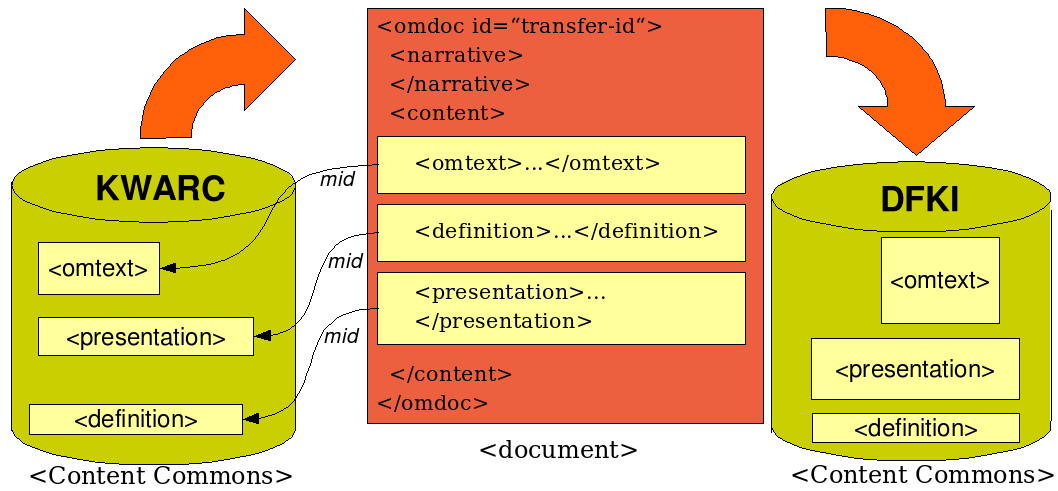
\includegraphics[width=0.5\textwidth]{img/interfaces.png}\vspace*{-1.5em}
%\caption{Documents as Interfaces}\label{fig:interfaces}
\end{wrapfigure} 
The figure on the right visualizes the idea of documents as interfaces to mathematical
knowledge. The {\infom}s in the {\emph{content commons}} of the {\emph{KWARC group}} are
embedded into an {\omdoc} document, in particular, they are cached in the
{\element{content}} element of an {\element{omdoc}} element, which in this case does not
necessarily include a {\element{narrative}} element. To make the references to the
oringinal {\infom}s, which are now (re-)used in the document,
{\emph{RESTful}}~\cite{wiki:rst}, unique, and aware of the used {\infom} state, we
re-introduce the {\omdoc}1.0 {\element{mid}} attribute. Each {\infom} within the
{\emph{content commons}} is keyed by a unique
{\tt{URI@REV}}\footnote{Subversion~\cite{SVN:web} calls {\tt{REV}} the peg revision to
  identify a unique line of history.} and can be requested by simple, stateless
{\sc{HTTP}} request ({\tt{PUT, POST, GET}} or {\tt{DELETE}}).  By this means, a document
may be used to transfer mathematical knowledge between {\emph{content commons}}, e.g.\
between the {\emph{KWARC}} and the {\emph{DFKI}} group.

%-----------------------------------------------------------------------------------------
\paragraph{Dependencies between Document and Content Commons:} 
\begin{wrapfigure}{r}{.5\textwidth}\vspace*{-.5em}
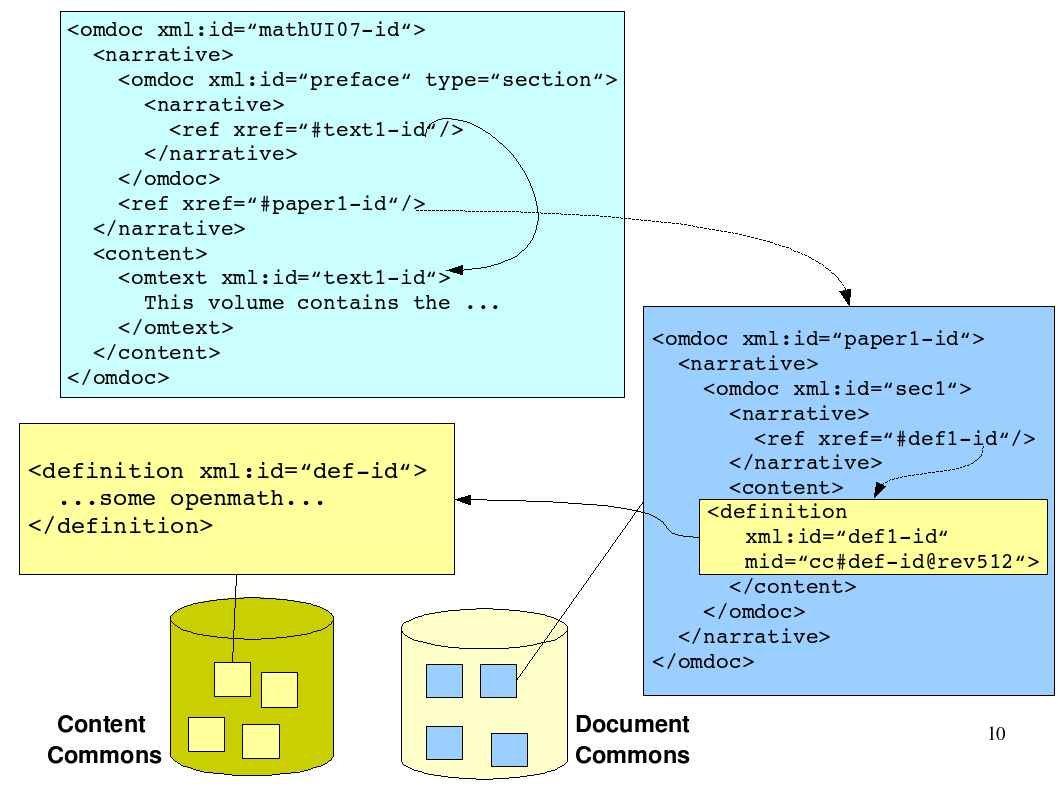
\includegraphics[width=.5\textwidth]{img/docsAndCommons.png}\vspace*{-.5em}
%\caption{Documents and Content Commons}\label{fig:docsAndCommons}
\end{wrapfigure}
Let us now consider the dependencies between a {\element{definition}} element in the
{\emph{content commons}}, a paper stored in the {\emph{document commons}}, and a currently
edited workshop proceedings. The {\element{narrative}} element of the proceedings
references the {\omdoc} representation of {\emph{paper1}}. The {\element{narrative}}
element further includes an {\element{omdoc}} child-element that references an
{\element{omtext}} element that is cached in the {\element{content}} element of the
proceedings and has not yet been stored in the {\emph{content commons}}. In contrast, the
{\element{narrative}} element of the paper references a {\element{definition}}, which is a
copy of an already existing and reused element from the {\emph{content commons}}. The
original {\element{definition}} is identified by the {\element{mid}} attribute of its
clone.


%-----------------------------------------------------------------------------------------
\paragraph{Narrative Structure and Content Management:}
\begin{wrapfigure}{r}{.5\textwidth}\vspace*{-1.5em}
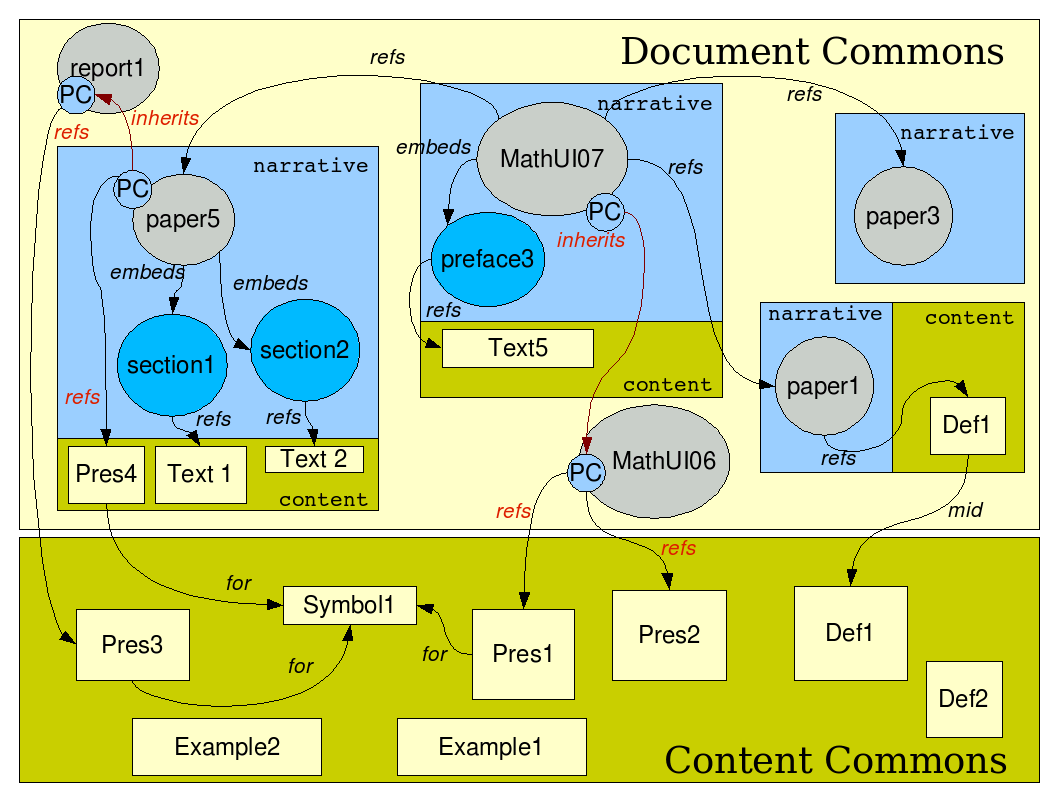
\includegraphics[width=.5\textwidth]{img/narcon.png}\vspace*{-.5em}
%\caption{Narrative Structure of the MKM-07 proceedings}\label{fig:narcon}
\end{wrapfigure}
The figure on the right displays the (cascading) narrative structure of the
{\emph{MathUI07 proceedings}}. The nodes of the {\emph{narrative graph}} references
{\element{omdoc}} elements in the {\emph{document commons}}, e.\,g.\ papers, or embed
{\element{omdoc}} child-elements specifying further narrative structures such as a
sections or paragraphs of a paper. The content of the {\element{omdoc}} elements is stored
in the sibling {\element{content}} elements and/ or the {\emph{content commons}}. For
example, the content of the {\emph{MathUI07}} and {\emph{paper5}} is only stored in their
local {\element{content}}, while the content of {\emph{paper1}} is stored in its local
{\element{content}} referencing the original {\infom} in the {\emph{content commons}}.
This also applies to {\element{presentation}} elements: The {\element{pcontext}} of the
{\emph{MathUI06 proceedings}} references {\element{presentation}} elements in the
{\emph{content commons}} which are not cached in the local {\element{content}} element,
while the referenced {\element{presentation}} element of {\emph{paper5}} is only stored in
its local {\element{content}}. In consequence, the content of documents may include copies
of the {\emph{content commons}}, but may also include new content that is not part of the
{\emph{content commons}}. In order to transfer a document independently from the
{\emph{content commons}}, its {\element{content}} element needs to cache all content of
the document.


%-----------------------------------------------------------------------------------------
\paragraph{Cascading Presentation Contexts and Prioritization:}

The cascading structure of the {\omdoc} representation of documents allows for the global
and local specification of presentation contexts: Each nodes of the narrative graph can be
associated with a specific {\element{pcontext}}, whereas the local {\element{pcontext}}
overwrite more general {\element{pcontext}}s. For example in the proceedings figure above,
the {\element{pcontext}} of the {\element{omdoc}} element representing the {\emph{MathUI07
    proceedings}} is inherited from the {\element{pcontext}} of the {\emph{MathUI06}}. The
{\element{pcontext}} of {\emph{paper5}} is implicitly inherited from the {\emph{MathUI06
    proceedings}} since the document is part of the narrative structure of the
{\emph{MathUI07 proceedings}}. Furthermore, it is extended by inheriting the
{\element{pcontext}} of {\emph{report1}} as well as a local reference to a
{\element{presentation}} element. The prioritization among {\element{pcontext}}s works as
follows: The local {\element{pcontext}} of {\emph{paper5}} overwrites the inherited
{\element{pcontext}} of {\emph{paper5}}, which further overwrites the implicitly inherited
{\element{pcontext}} of {\emph{MathUI07 proceedings}}: In particular, the prioritization
of the presentation for {\emph{symbol1}} are: {\emph{Pres1}}, which is overwritten by
{\emph{Pres3}}, which is further overwritten by the locally referenced {\emph{Pres4}} with
the highest priority.

The prioritization on {\element{omdoc}} element level provides authors with the following
options: They can either manually specify all the {\element{presentation}}s, which
consequently leads to rather {\emph{static document}}. Alternatively, they can choose to
omit most of the presentation specification, which leads to {\emph{flexible documents}}
that can be embedded in the {\element{pcontext}} of other documents. For example, while
{\emph{paper5}} overwrites the inherited {\element{pcontext}} of the proceedings,
{\emph{paper1}} adopts the referenced {\element{presentation}} elements.

The following listings provides the {\omdoc} representation of the {\emph{MathUI07
proceedings}}. In addition to the {\emph{preface}} and the referenced papers, the
{\element{narrative}} of the {\emph{proceedings}} includes two special elements,
i.e.\ a {\emph{table of contents}} and an {\emph{author index}}:
\begin{lstlisting}[mathescape,caption={Representation of the MathUI
proceedings},label=lst:MathUIproceedings]
<omdoc xml:id="mathUI07" type="proceedings">
  <pcontext xml:id="pc-mathUI07" base="#mathUI06"/>
  <narrative>
    <metadata><dc:title>MathUI07</dc:title></metadata>
    <omdoc xml:id="preface" type="preface">
      <narrative>
        <metadata><dc:title>Preface</dc:title></metadata>
        <ref xref="#text5"/>
      </narrative>
    </omdoc>
    <tableofcontents/>
    <ref xref="#paper1"/><ref xref="#paper3"/><ref xref="#paper5"/>
    <authorindex/>
  </narrative>
  <content>
    <omtext xml:id="text5"><CMP>This volume contains the proceedings of the...</CMP></omtext>
  </content>
</omdoc>
\end{lstlisting}

The {\omdoc} specification below represents {\emph{paper5}} of the {\emph{MathUI07}}: It
inherits its presentation context from the proceedings {\element{pcontext}}, but extends/
overwrite it by the inherited {\element{pcontext}} of the referenced report and a local
reference to a {\element{presentation}} element.

\begin{lstlisting}[mathescape] 
<omdoc xml:id="paper5" type="paper">
  <pcontext xml:id="paper5-pc" base="#report-pc"><ref xref="#pres4-id"/></pcontext>
  <narrative>
    <metadata><dc:title>Documents with flexible Notation Contexts as Interfaces to Mathematical Knowledge</dc:title></metadata>
    <omdoc xml:id="section1" type="section">
      <narrative>
        <metadata><dc:title>Introduction</dc:title></metadata> <ref xref="#text1"/>
      </narrative>
      <content>
        <omtext xml:id="text1">
          <CMP>In this paper we explore the use of documents as interfaces to mathematical knowledge.</CMP>
        </omtext>
      </content>
    </omdoc>
    <omdoc xml:id="section2" type="section">
      <narrative>
        <metadata><dc:title>Outlook</dc:title></metadata>
        <ref xref="#text2"/>
      </narrative>
      <content><omtext xml:id="text2"><CMP>To sum up ...</CMP></omtext></content>
    </omdoc> 
  </narrative>
  <content><presentation xml:id="pres4-id">...</presentation></content>
</omdoc>
\end{lstlisting}


%-----------------------------------------------------------------------------------------
\paragraph{Presentation Contexts within {\omdoc} elements:}
The association of presentation contexts to narrative nodes is one way to specify the
presentation context. However, in some cases this is not sufficient, requiring for a more
local specification: In {\omdoc} this is solved by extending the {\element{phrase}} and
{\element{ref}} element with an optional attribute {\attribute{pc}{*}} that references the
respective {\element{presentation}} element. Please note that the presentation contexts
given by {\attribute{pc}{*}} attributes overwrites the specification in the
{\element{pcontext}} elements: For example in listing~\ref{lst:multicontext}, the
{\attribute{pc}{*}} attributes, which references the {\element{presentation}} element for
the French $C_{k}^n$ and Russian $C_{n}^k$ notation, overwrite the more global
specification in the {\element{pcontext}}, i.e. the German presentation ${n \choose k}$.

\begin{lstlisting}[mathescape,caption={A Multi-context
Presentation},label=lst:multicontext]
<omdoc xml:id="section3" type="section">
  <narrative>
    <omdoc type="para">
      <pcontext xml:id="pc1"><ref xref="#bk-D"/><pcontext>
      <narrative><ref xref="#text1"/></narrative>
      <content>
        <omtext xml:id="text1">
          <CMP>We will discuss the binomial coefficient which can be represented in three alternative ways: i.e. 
          <OMOBJ xml:id="foo">
            <OMA><OMS cd="bk" name="bk"/><OMV name="n"/></OMV name="k"/></OMA>
          </OMOBJ> (Germany), 
          <ref xref="#foo" pc="#bk-F"/> (France), and <ref xref="#foo" pc="#bk-R"/> (Russia) </CMP>
        </omtext>
      </content>
    </omdoc>
  </narrative>
</omdoc>
\end{lstlisting}

After transforming the {\omdoc} representation into PDF, the original document would
appear as shown below:
\begin{figure}[ht]
\begin{center}
\fbox{\begin{minipage}{0.8\textwidth}
We will discuss the binomial coefficient which can be represented in three alternative
ways: i.e. ${n \choose k}$ (Germany), $C_{k}^n$ (France), and $C_{n}^k$ (Russia).
\end{minipage}}
\caption{The presentation of listing~\ref{lst:multicontext}}
\end{center}
\end{figure}
\vspace*{-1.cm}

%%%%%%%%%%%%%%%%%%%%%%%%%%%%%%%%%%%%%%%%%%%%%%%%%%%%%%%%%%%%%%%%%%%%%%%%%%%%%%%%%%%%%%%%%%
\section{Conclusion and Future Work}\label{sec:outlook}

In this paper we have initiated the redefinition of {\emph{documents}} towards a more
{\emph{dynamic}} and {\emph{living}} view. So far, the term mostly referred to static
articles and publications, neglecting the new opportunities offered by modern
technologies.  In the first step, we have explicated the narrative and content layer and
extended the {\emph{document model}} by a third dimension, i.e. the presentation layer. We
further specified how the notation contexts of a document can be modeled on different
cascading layers, i.e. on the {\element{omdoc}} element level by using
{\element{pcontext}} elements as well as within {\element{omdoc}} elements by specifying
{\attribute{pc}{*}} attributes. However, several issues remain, which we will address in
future work:


%-----------------------------------------------------------------------------------------
\paragraph{Personalization of Documents:} The specification of a document's notation
context can be used to automatically adapt the presentation to a specific (personalized)
context, e.\,g.\ of a group or user. However, this requires to {\emph{prioritize the
    context specifications}}, which is not trivial: We already mentioned, that within the
cascading structure of documents a local {\element{pcontext}} overwrite a more global
{\element{pcontext}}; and the {\attribute{pc}{*}} attribute overwrites the
{\element{pcontext}} of the {\element{omdoc}} element. However, the prioritization of a
document's notation contexts among various contexts, such as system default, the author's
and group's notation context as well as the individual (reader's) contexts has not been
sufficiently solved yet.

For example, applying the prioritization in~\cite{ManLib:apo05} takes away the intention
of the author: If we allow a user to overwrite the presentation context in
listing~\ref{lst:multicontext} by his individual style, i.e.\ the German presentation of
the binomial coefficient, the adaptation would end in nonsense:

\begin{figure}[ht]
\begin{center}
\fbox{\begin{minipage}{0.8\textwidth}
We will discuss the binomial coefficient which can be represented in three alternative
ways: i.e. ${n \choose k}$ (Germany), ${n \choose k}$ (France), and ${n\choose k}$
(Russia).
\end{minipage}}
\caption{A nonsensical presentation of listing~\ref{lst:multicontext}}
\end{center}
\end{figure}
\vspace*{-.5cm} We are currently working on supporting authors to preserve specific
notations, i.e.\ to indicate whether a presentation can be adapted or not. One possible
way is to add priorities to the presentation contexts as e.g. in {\css} or {\xslt}.


%-----------------------------------------------------------------------------------------
\paragraph{Extensional vs. Intensional Model:} In the first step we use an
{\emph{extensional model}} to specify the notation context, i.e.\ the author has to
specify all presentations for symbols in his document by either inheriting existing
specifications or referencing {\element{presentation}} elements. In the next step, we will
also evaluate and potentially model an {\emph{intensional approach}}, i.e.\ the author
will be enabled to specify a context by e.g.\ indicating the language, the area of
application, or the level of sophistication. His intensional specification will then
trigger an automatic identification of {\element{presentation}} elements for symbols in
his document. One possible way to support the intensional specification is adding
{\attribute{type}{presentation}} attributes to the {\element{presentation}} element
(cf.~\cite{ManLib:apo05}). For example, the type {\attval{de}{type}{presentation}}
specifies German presentations, {\attval{physics}{type}{presentation}} specifies
presentation for symbols in physics, or {\attval{elementary-level}{type}{presentation}}
indicates the level of sophistication. In order to allow for a more flexible specification
in {\omdoc}2.0, the syntax of {\element{presentation}} elements has been respecified
in~\cite{KohLanRab:pmcfe07}.


%-----------------------------------------------------------------------------------------
\paragraph{From Notation Contexts to {\cop} Models:} 
We have extended the specification of notation context and practice by our predecessors,
e.\,g.\ Watts/Smirnova~\cite{ESmStW:Notation} and {\activemath}~\cite{ManLib:apo05},
towards a more general model: Instead of predefining system defaults, a book's or an
author's context, we provide a model that allows for {\emph{reusability}} of existing
contexts, e.\,g.\ of a paper or book. In the next step, we aim at providing means to
specify the notation context of an individual and communities of practice.

One potential mean to specify an author's or {\cop} notation context is using
{\element{omdoc}} elements as a collection of references to their preferred or {\emph{most
    frequently used}} presentations. The following listing provides an example for such an
{\element{omdoc}} element. The {\element{pcontext}} of the document references the
{\element{presentation}} elements used for symbols within the document written by the
author or {\cop}. For example, the author ``Christine Mueller'' has used symbols of the
\emph{MathUI06}, a \emph{report}, and a \emph{specific} {\element{presentation}}
element. The respective {\element{presentation}} elements are stored in the content
commons and/ or the {\element{content}} element of the document.

\begin{lstlisting}
<omdoc xml:id="cmueller-pcontext" type="notationcontext">
  <narrative>
  <metadata><dc:title>The notation context of Christine Mueller</dc:title></metadata>
  <narrative>
  <pcontext><ref xref="#mathUI06"/><ref xref="#report"/><ref xref="#pr4"/><pcontext>
  <content>
    <presentation xml:id="pr4" for="#bk" role="applied">
      <use format="TEX" lbrack="\bigl({" rbrack="}\bigr)">\atop</use>
      <use format="pmml" element="mfrac" attributes="linethickness='0'"/>
      <use format="default" fixity="infix">choose</use>
    </presentation>
  </content>
</omdoc>
\end{lstlisting}

The identification of {\cop}s can be based on an analysis of a collection of notation
contexts gained from a document collection. For now, the identification of a {\cop}'s
notation contexts is simply a prioritized merge of all {\element{pcontext}} elements and
{\attribute{pc}{*}} attributes of their documents. However, we took the first step towards
a concrete application of the theory of {\emph{communities of practice}} towards a
scientific and technical field. We are currently working on an improved method for
establishing {\cop}s, e.g. by means of an cluster analysis to identify the {\cop}'s most
frequently used presentations.

The identification of individual contexts is analogous: In the beginning, authors will
manually specify their preferred presentation context. We will then implement routines
that automatically detect an author's preferred notations. In order to store an author's
notation contexts we propose the implementation of
{\emph{ePortfolio}}s\footnote{ePortfolios are digital collections of private documents,
  such as individual notation contexts or {\cop} information.}. We are currently
developing an educational platform that manages ePortfolios of students, which will be use
to evaluate the specification and deployment of notation contexts as well as to take
further steps towards a scientific {\cop} model.

\paragraph{Acknowledgments}\label{sec:ack}
We would like to thank the other members of our KWARC group for the fruitful discussions
and continuous feedback on our work.



%%%%%%%%%%%%%%%%%%%%%%%%%%%%%%%%%%%%%%%%%%%%%%%%%%%%%%%%%%%%%%%%%%%%%%%%%%%%%%%%%%%%%%%%%%
\begin{footnotesize}
\bibliography{kwarc} 
\bibliographystyle{alpha}
\end{footnotesize}
\end{document}
%%% Local Variables: 
%%% mode: latex
%%% fill-column: 90
%%% End: 

% LocalWords:  {\cop} {\cop}s co sind Dokumente einem kontentgetriebenen Kontext wie
% LocalWords:  repaesentieren wir Dokumenten nicht und ist vollstaendig Fokus
% LocalWords:  NarCon Struktur Verbindung mit Praesentation MathWebSearch {\xslt}
% LocalWords:  Naylor Manzoor al schon bekannt dem Leser hilft achste Sektion
% LocalWords:  zu verstehen das Smirnova priorization MathWebWiki Normen uller
% LocalWords:  nar rative Infoms Struktuerierung Uebergang passt Respecifying
% LocalWords:  omdoc pcontext resentation ontext xml xsd NCName xref anyURI ref
% LocalWords:  omtext {\cop}'s docsAndCommons narcon openmath mathescape mkm dc pc
% LocalWords:  CMP para bk OMOBJ foo OMA OMS cd OMV PDF cmueller CMueller pres
% LocalWords:  notationcontext pr lbrack rbrack pmml mfrac linethickness fixity
% LocalWords:  de doc JEM Stamerjohanns ePortfolios Christoph Florian Rabe PO
% LocalWords:  kwarc omgroup att anyURIs tableofcontents authorindex URI lst CR
% LocalWords:  RESTful MathUIproceedings mathUI multicontext bibtex faellt dir
% LocalWords:  ein Automization steckt oben mal drin aber ich weiss hier noch
% LocalWords:  schreiben soll sgml LD
